% +----------------------------------------------------------------------------+
% | Instituto Nacional de Pesquisas Espaciais - INPE
% | ----------------------------------------------------------------------------
% | Authors     : M. E. G. Borges; M. L. S. Nascimento; J. E. C. Cruz
% | Version     :
% | Copyright   :
% | Description : Registro e Mosaico de Imagens Obtidas por VANTs
% +----------------------------------------------------------------------------+

\documentclass[9pt, a4paper, nofonttune, journal]{IEEEtran}
\usepackage[utf8x]{inputenc}
\usepackage[T1]{fontenc} % permite copiar texto com acento em PDF
\usepackage{url}
\usepackage{graphicx}
\usepackage{amsmath}%pacote necessário para a utilização de algumas funções matemáticas nas formulas
\usepackage{float}%responsável por o posicionamento de figuras

% correct bad hyphenation here
\hyphenation{pro-ble-mas mosaico}


\begin{document}

\title{Registro e Mosaico de Imagens \\Obtidas por Câmera Digital a bordo de VANT}

\author{
  \IEEEauthorblockN{
    Marcos Eduardo Gomes Borges \IEEEauthorrefmark{1}\\
    Marina Laís da Silva Nascimento \IEEEauthorrefmark{1}\\
    Juliano E. C. Cruz \IEEEauthorrefmark{1}\\
    Leila Maria Garcia Fonseca \IEEEauthorrefmark{2} \linebreak\linebreak
  }
  \IEEEauthorblockA{
    Instituto Nacional de Pesquisas Espaciais – INPE\\
    Programa de Mestrado em Computação e Matemática Aplicada \IEEEauthorrefmark{1}\\
    Divisão de Processamento de Imagens \IEEEauthorrefmark{2}\\
    São José dos Campos, Brasil\\
    \{marcoseborges, marina.lsnascimento, juliano.ecc\}@gmail.com, leila@dpi.inpe.br
  }
}

% The paper headers
\markboth{Journal of DPI-INPE,~Vol.~XX, No.~1, Janeiro~2012}%
{Shell \MakeLowercase{\textit{et al.}}: Trabalho de PDI - INPE}

\maketitle               
\renewcommand\abstractname{Resumo}
\renewcommand{\refname}{Referências}
\renewcommand\IEEEkeywordsname{Palavras-chave}


\begin{abstract}
Neste trabalho foi pesquisado soluções para registro e mosaico de imagens adquiridas por câmera digital a bordo de VANT. A ideia é apresentar soluções para dois tipos de problemas que ocorrem ao mosaicar sequências de imagens aéreas: i) distorções geométricas inseridas na imagens devido às variações de altitude, ii) distorções (escala, projeção e ângulo de visada) nas imagens de baixas altitudes e que possuem cenas de objetos altos, tais como prédios e montanhas.
\end{abstract}

\begin{IEEEkeywords}
Registro de Imagens, Mosaico, VANT, TerraLib, SIFT.
\end{IEEEkeywords}

\section{Introdução}
A utilização de Veículos Aéreos não Tripulados (VANTs) tem apresentado grande crescimento nos últimos anos devido a diversos fatores, 
tais como ausência de tripulação em tarefas tediosas, cansativas ou que envolvem riscos à tripulação, 
baixo custo operacional e de fabricação comparados às aeronaves convencionais, entre outros. 
Imagens aéreas obtidas através de VANTs possuem grandes aplicabilidades \cite{Canhoto}
 e o objetivo geral deste trabalho é encontrar solução para distorções geométricas que surgem ao realizar registro e mosaico de imagens adquiridas por câmera digital a bordo de aeronaves não tripuladas.

O mosaico de sequências de imagens aéreas apresenta alguns problemas de distorções geométricas devido às variações de altitudes da aeronave e 
distorções devido as diferenças de escala, projeção e ângulo de visada em cenas de baixa altitude e que apresentam prédios e montanhas. 
Outro problema também enfrentado ao mosaicar esse tipo de imagem, 
é que quando a aeronave realiza curvas para seguir o plano de voo traçado captura imagens com sistema de coordenadas rotacionadas em ângulos diferentes e desconhecidos, 
e isso também gera distorções que buscamos resolver neste trabalho.

Na Figura~\ref{fig:plano_voo} pode-se observar o exemplo de um plano de voo para um VANT. 
Neste trabalho, as imagens adquiridas pela câmera digital a bordo da aeronave não possuem georeferenciamento e são coletadas a cada um segundo. 
Após o término da aquisição das imagens, as mesmas necessitam ser mosaicadas. 
O procedimento inicial para essa tarefa é o registro de imagens, que inicia a busca por correspondências entre imagens diferentes que representam a mesma cena \cite{Goltz:08}. 
Neste trabalho, a busca por correspondências entre pontos de imagens diferentes é realizada e comparada entre os algoritmos: SIFT proposto por \cite{Lowe} 
e pelos algoritmos de registro implementados na biblioteca TerraLib.

\begin{figure}[h!t]
  \centering
  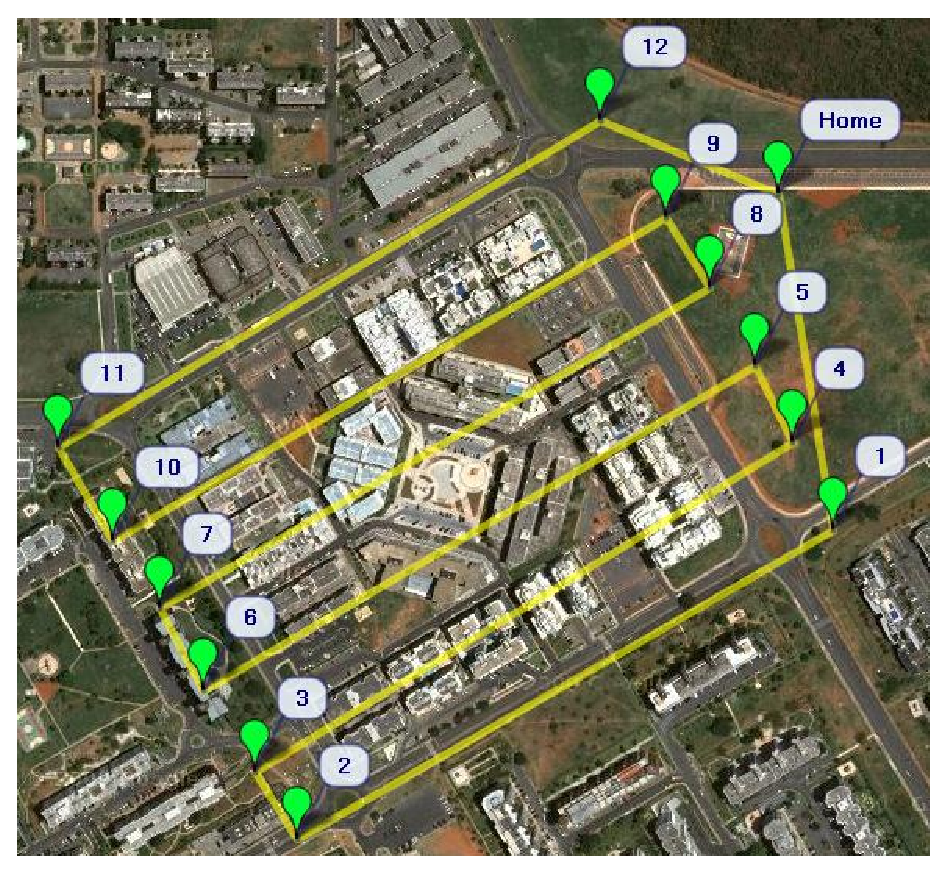
\includegraphics[width=3.3in]{figuras/plano_voo}
  \caption{Exemplo de Plano de Voo do VANT}
  \label{fig:plano_voo}
\end{figure}

\section{Registro e Mosaico de Imagens}
O registro de imagens pode ser entendido como um processo de casamento entre duas imagens que possuem uma área comum.
A imagem tomada como base de registro é chamada de imagem de referência, e a imagem a ser registrada é chamada de imagem de ajuste.
O processo basicamente envolve três etapas:
\begin{enumerate}
	\item Obtenção de pontos de controle;
	\begin{enumerate}
		\item Extração de feições;
		\item Casamento das feições extraídas;
	\end{enumerate}
	\item Determinação da função de transformação;
	\item Sobreposição das imagens.
\end{enumerate}

As imagens a serem registradas podem ser relacionadas atavés de função de transformação simples se a geometria das imagens for semelhante.
Se a geometria das imagens for diferente, as transformações podem ser aproximadas utilizando um função polinomial cujos parâmetros são determinados 
a partir das coordenadas dos pontos de controle.
O número de pontos de controle representa a situação de um sistema de equações determinado.
Entretanto, como as coordenadas medidas dos pontos de controle estão sujeitas a erros, convém usar um número de pontos maior que o número mínimo,
o que define um sistema de equações sobredeterminado.

O produto gerado através das técnicas de registro de imagens é o mosaico, que nada mais é do que uma 
composição de imagens adquiridas de diferentes pontos de vista visando contruir uma imagem maior, permitindo assim uma visão global da cena.\cite{Fedorov1}

\section{Ferramentas}
Para se realizar os processos de registro citados anteriormente, foram utilizadas duas ferramentas.

\subsection{TerraLib}
TerraLib é uma biblioteca \textit{open source} de classes e funções SIG disponível na Internet, possibilitando portanto um ambiente colaborativo e seu uso
para o desenvolvimento de novas ferramentas. Assim, deseja-se possibilitar uma nova geração de aplicações SIG baseada nos avanços tecnológicos dos bancos de dados espaciais.
A TerraLib é desenvolvida pela DPI, divisão pertencente ao INPE, Tecgraf, PUC-Rio e FUNCATE.\cite{Terralib1}


\subsection{SIFT}

O algoritmo SIFT - Scale Invariant Feature Transform foi desenvolvido por [1] em 1999 e sua função é construir descritores de pontos-chaves de uma imagem,
 sendo este descritores independentes das mudanças de escala, rotação, translação e luminosidade que uma imagem pode sofrer.
Utilizamos neste trabalho a implementação em C++ obtida em \cite{Vedaldi}.
O SIFT é utilizado na busca por correspondências entre sequência de imagens diferentes que contenham partes da mesma cena. 
A busca é feita através de pontos-chave correspondentes, utilizando-se seus descritores. 
Nesta pesquisa a distância euclidiana é utilizada em três abordagens diferentes para avaliar a mais apropriada para imagens obtidas por VANTs. 
Os algoritmos de cada abordagem são: DistEuclidConvencional, o qual aplica a função de busca diretamente, sem tratar seus resultados. 
DistEuclidRedundante, que chama a função de busca duas vezes, a segunda chamada é feita invertendo-se os parâmetros da função, 
somente correspondências que ocorram em ambas são guardadas. 
DistEuclidEsc onde observa-se a continuidade de escala entre segmentos de reta traçados entre os pontos pertencentes e às correspondências geradas 
por esta função.

\section{Detecção de pontos de interesse}
Ponto de interesse é como é chamado qualquer ponto de uma imagem em que o sinal mude bidimensionalmente. Cantos ou ângulos
no formato L, T e Y obecem essa definição assim como pontos pretos em um fundo branco, o final de ramificações ou qualquer textura bidimensional
significante.\cite{Coderlia1}

Os algoritmos que serão descritos subsequentemente são utilizados por duas classes do TerraLib:
\texttt{TePDIMMIOMatching} utiliza o operador Moravec e \texttt{TePDIOFMatching} utiliza o método de fluxo ótico.
\subsection{Detector Moravec}
O operador Moravec foi uma dos primeiros detectores de ponto de interesse a serem desenvolvidos, sendo descrito primeiramente 
em 1977 por Hans Moravec.\cite{Moravec1}
Esse operador é baseado na função de auto-correlação do signal. Ele compara as diferenças de nível de cinza entre a janela atual e de janelas 
deslocadas em quatro direções paralelas à colunas e linhas. Se o mínimo dessas quatro diferenças é superior a um determinado limiar, então um ponto de interesse
foi encontrado.\cite{Coderlia1}
  
O operador Moravec pode ser definido matematicamente como:
    \begin{center}$V_{1}=\frac{1}{p(q-1)}\sum_{i=-k}^k\sum_{j=-l}^{l-1}\bigl(g(i,j)-g(i,j+1)\bigr)^2$    \end{center}
    \begin{center}$V_{2}=\frac{1}{(p-1)q}\sum_{i=-k}^{k-1}\sum_{j=-l}^l\bigl(g(i,j)-g(i+1,j)\bigr)^2$    \end{center}
    \begin{center}$V_{3}=\frac{1}{(p-1)(q-1)}\sum_{i=-k}^{k-1}\sum_{j=-l}^{l-1}\bigl(g(i,j)-g(i+1,j+1)\bigr)^2$\end{center}
    \begin{center}$V_{4}=\frac{1}{(p-1)(q-1)}\sum_{i=-k}^{k-1}\sum_{j=-l}^{l-1}\bigl(g(i,j+1)-g(i+1,j)\bigr)^2$\end{center}
    \begin{center}$V = min(V1,V2,V3,V4)$\end{center}

    Onde $p = 2k + 1$ e $q = 2l + 1$, sendo que $k\times l$ é o tamanho da janela utilizada. 

\subsection{Fluxo Ótico}
Fluxo ótico é a distribuição de velocidades aparentes do movimento de padrões de brilho em uma imagem \cite{GibsonBook1}. Assim, pode-se obter informações importantes a respeito da distribuição espacial dos objetos visualizados 
e da taxa de mudança dessa distribuição. Discontinuidades do fluxo ótico podem ajudar a segmentar uma determinada imagem 
em regiões que correspondem a diferentes a diferentes objetos.
Esse conceito começou a ser estudado na década de 1940 e foi publicado primeiramente pelo psicólogo americano James Gibson \cite{Gibson1} \cite{OF1}.

Um pixel tendo a localização $(x,y,t)$ com intensidade $I$ será movido em $\Delta x$,$\Delta y$ and $\Delta t$ entre os quadros de uma mesma imagem.
Assim, chega-se a equação:

\begin{center}
$\frac{\partial I}{\partial x}\frac{\Delta x}{\Delta t}+\frac{\partial I}{\partial y}\frac{\Delta y}{\Delta t}+\frac{\partial I}{\partial t}\frac{\Delta t}{\Delta t} = 0 $\end{center}
simplificando tem-se que,
\begin{center}
$\frac{\partial I}{\partial x}V_x+\frac{\partial I}{\partial y}V_y+\frac{\partial I}{\partial t} = 0$\end{center}
Onde $V_x$ e $V_y$ são os componentes $x$ e $y$ do fluxo ótico.


\section{Casamento de pontos de interese}
Após se obter os pontos de interesse de ambas as imagens em que deseja-se realizar o registro,
é necessário descobrir qual é o ponto da imagem de referência que é o correspondente à um determinado ponto na imagem de ajuste. 

Dentre diversos métodos existentes para se descobrir a correspondência entre os pontos, as classes de casamento do TerraLib utilizam
o método estatístico de correlação cruzada normalizada.
Seu funcionamento se dá ao extrair pequenas janelas ao redor de cada ponto de interesse nas duas imagens.
Aplica-se , então, aos pares o método(descrito abaixo) entre todas as janelas obtidas na imagem de referência com as obtidas na imagem de ajuste.\cite{Fedorov1}\cite{Leila1}\cite{Zhao1}
\begin{center}
$R(i,j)=\frac{\overset{K-1}{\underset{l=0}{\sum}}\underset{m=0}{\overset{L-1}{\sum}}W_{z}(l,m)\cdot S_{ij}(l,m)}{\sqrt{\overset{K-1}{\underset{l=0}{\sum}}\underset{m=0}{\overset{L-1}{\sum}}W_{z}^{2}(l,m)\overset{K-1}{\underset{l=0}{\sum}}\underset{m=0}{\overset{L-1}{\sum}}S_{ij}^{2}(l,m)}}$\end{center}
Onde $S_{ij}$ é a janela da imagem de referência e $W_{z}$ a janela da imagem de ajuste.
Assim, o maior valor de $R(i,j)$ significa que as duas janelas comparadas são as mais parecidas.



\section{Transformadas Geométricas}
Transformação geométrica é o nome que se dá à aplicação de uma determinada função matemática em uma determinada figura geométrica 
em que o resultado é geometricamente igual ou semelhante à figura original.

\subsection{Transformações elementares}
\subsubsection{Translação}
A translação desloca um determinado ponto ou conjunto de pontos uma determinada distância em um determinado sentido.

\begin{center}
$\begin{bmatrix}x'\\
y'
\end{bmatrix}=\begin{bmatrix}x\\
y
\end{bmatrix}+\begin{bmatrix}t_{x}\\
t_{y}
\end{bmatrix}$\end{center}
Onde $t_{x}~~ \textrm{e} ~~ t_{y}$ são respectivamente as taxas de translação no eixo $x~~ \textrm{e} ~~y$.\cite{CGPPBook1}


\begin{figure}[H]
\begin{center}
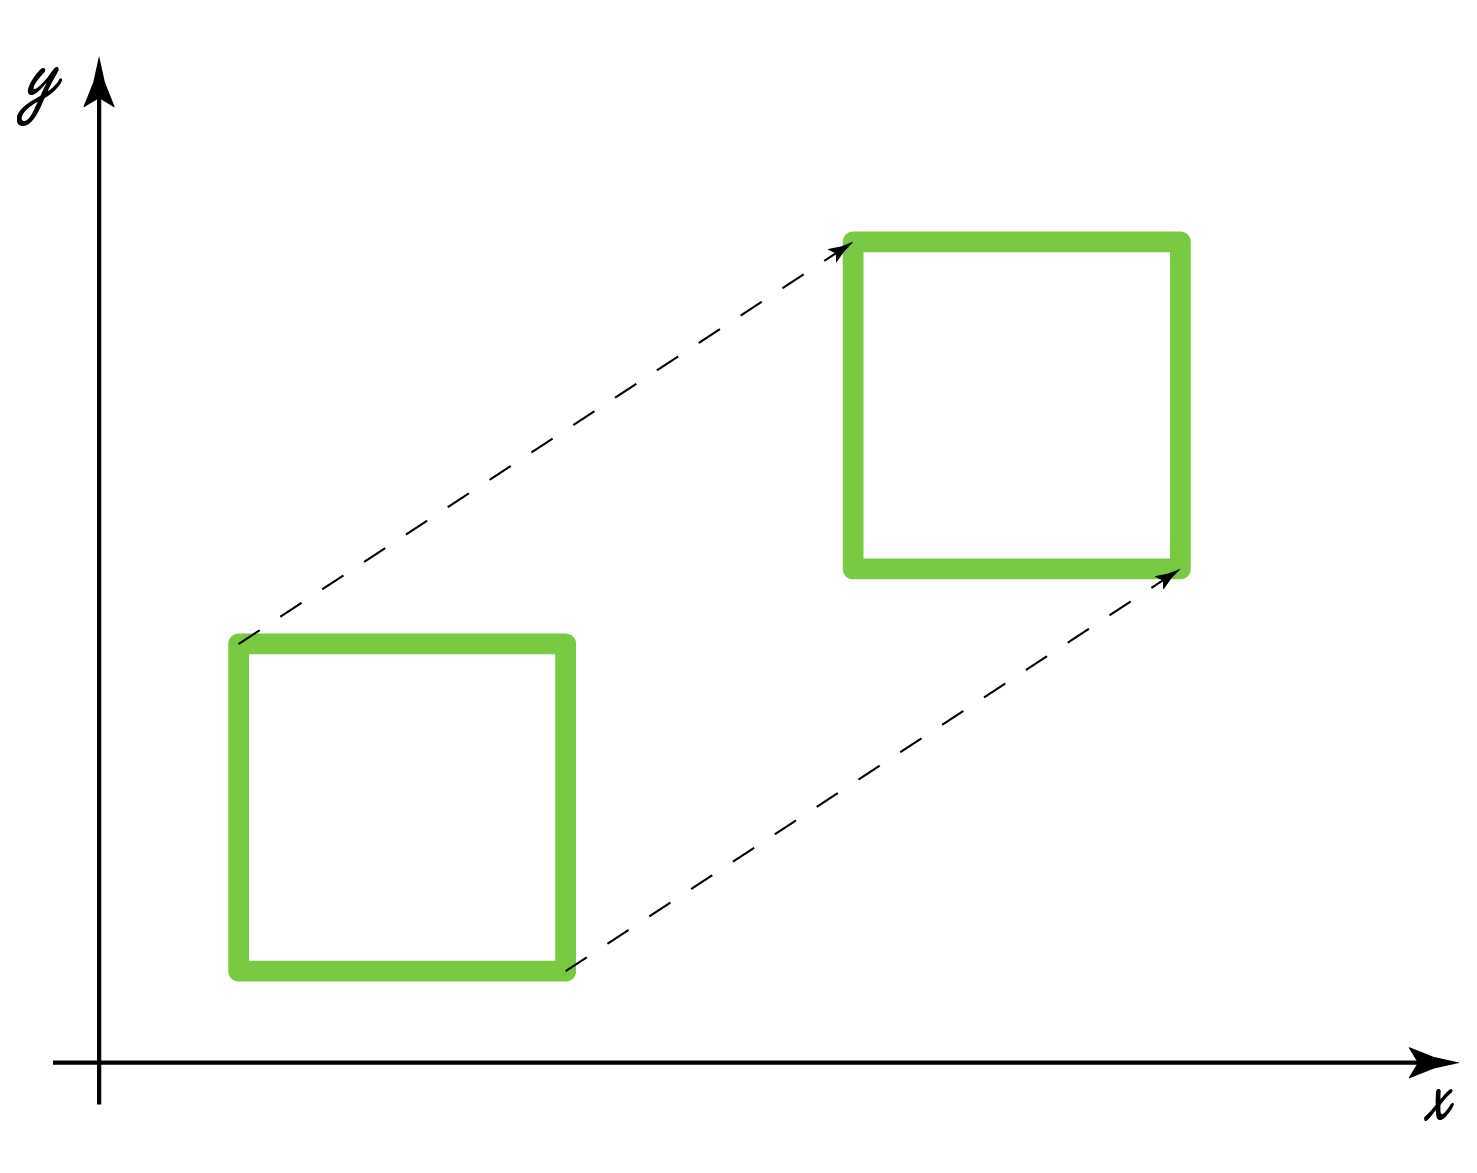
\includegraphics[scale=0.25]{figuras/translation1}
\caption{Exemplo de translação em um espaço bidimensional}
\end{center}
\end{figure}

\subsubsection{Variação de escala}

A variação de escala é o fato de se esticar ou encolher uma determinada figura em relação ao eixos $x$ e $y$.

\begin{center}
$\begin{bmatrix}x'\\
y'
\end{bmatrix}=\begin{bmatrix}v_{x} & 0\\
0 & v_{y}
\end{bmatrix}\begin{bmatrix}x\\
\frac{}{}y
\end{bmatrix}$\end{center}
Onde $v_{x}~~ \textrm{e} ~~ v_{y}$ são respectivamente as taxas de escala no eixo $x~~ \textrm{e} ~~y$.\cite{CGPPBook1}


\begin{figure}[H]
\begin{center}
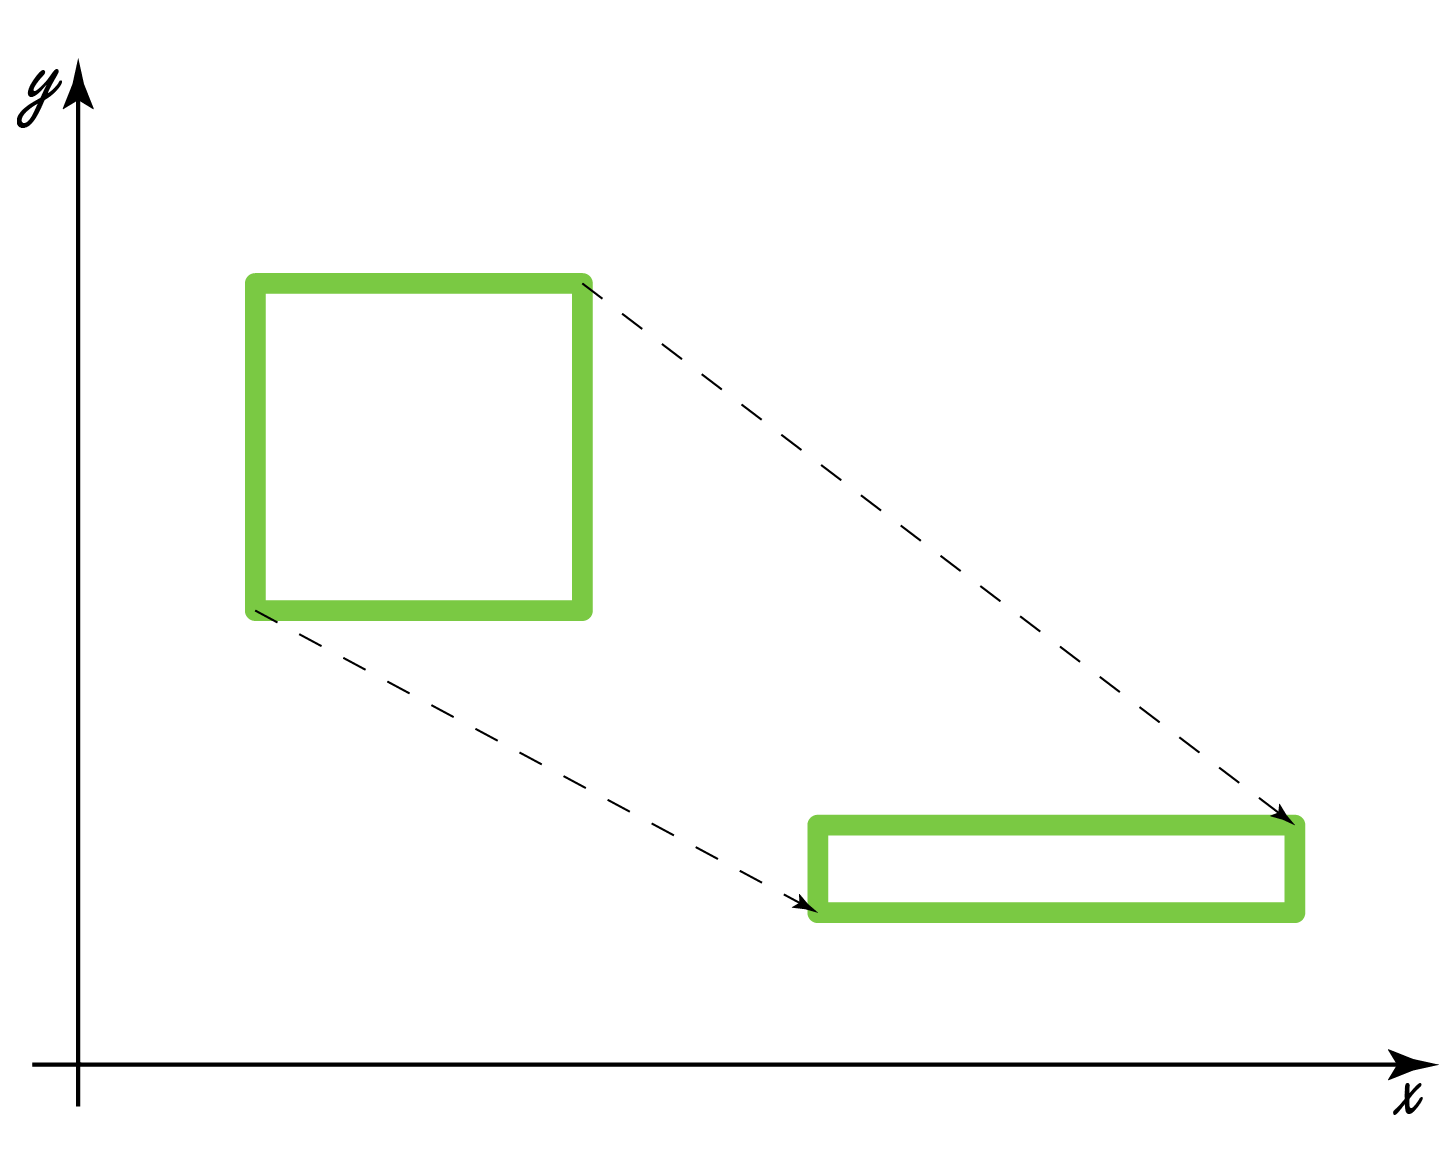
\includegraphics[scale=0.25]{figuras/scale1}
\caption{Exemplo de variação de escala em um espaço bidimensional}
\end{center}
\end{figure}

\subsubsection{Rotação}
Na rotação rotaciona-se a figura em torno de um determinado eixo.

\begin{center}
$\begin{bmatrix}x'\\
y'
\end{bmatrix}=\begin{bmatrix}cos\theta & -sen\theta\\
cos\theta & sen\theta
\end{bmatrix}\begin{bmatrix}x\\
y
\end{bmatrix}$\end{center}
Onde $\theta$ é o ângulo que a figura será rotacionada em relação a posição original levando em consideração a origem como eixo. \cite{CGPPBook1}

\begin{figure}[H] 
\begin{center}
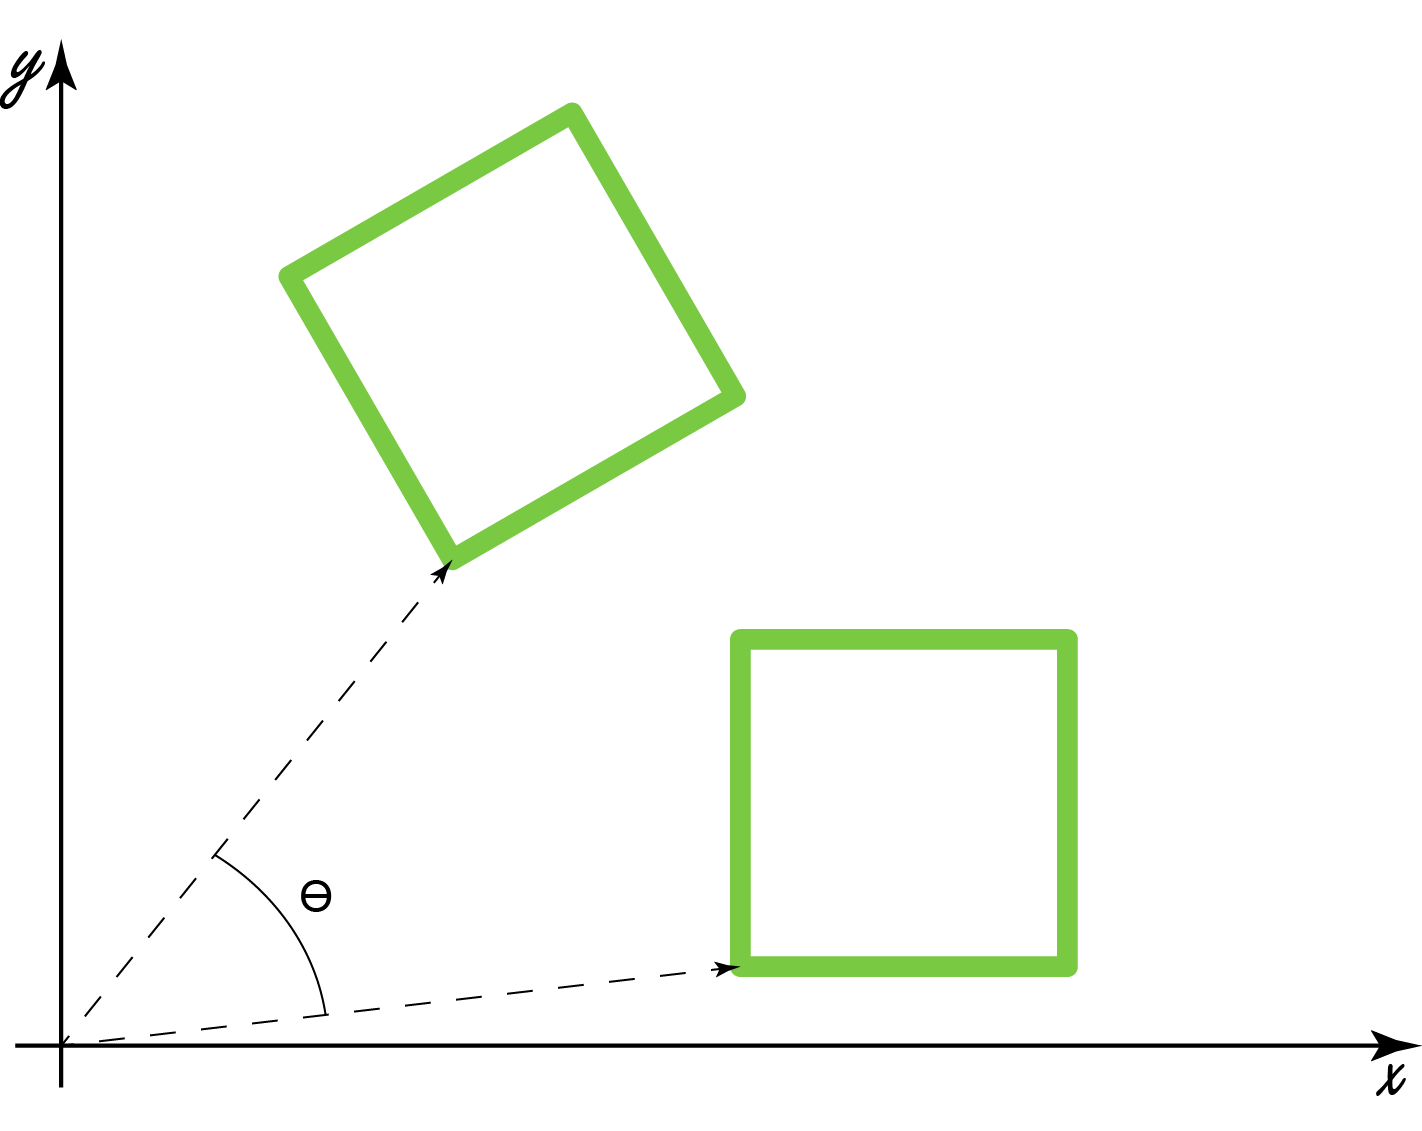
\includegraphics[scale=0.25]{figuras/rotation1}
\caption{Exemplo de rotação em um espaço bidimensional}
\end{center}
\end{figure}

\subsubsection{Cisalhamento}
O cisalhamento resulta em um movimento translacional na direção de um eixo no qual a magnitude aumenta ao longo do outro eixo.

\begin{center}
$\begin{bmatrix}x'\\
y'
\end{bmatrix}=\begin{bmatrix}1 & c\\
1 & 0
\end{bmatrix}\begin{bmatrix}x\\
y
\end{bmatrix}$\end{center}
Onde $c$ é o coeficiente de cisalhamento.\cite{CGPPBook1}

\begin{figure}[H] 
\begin{center}
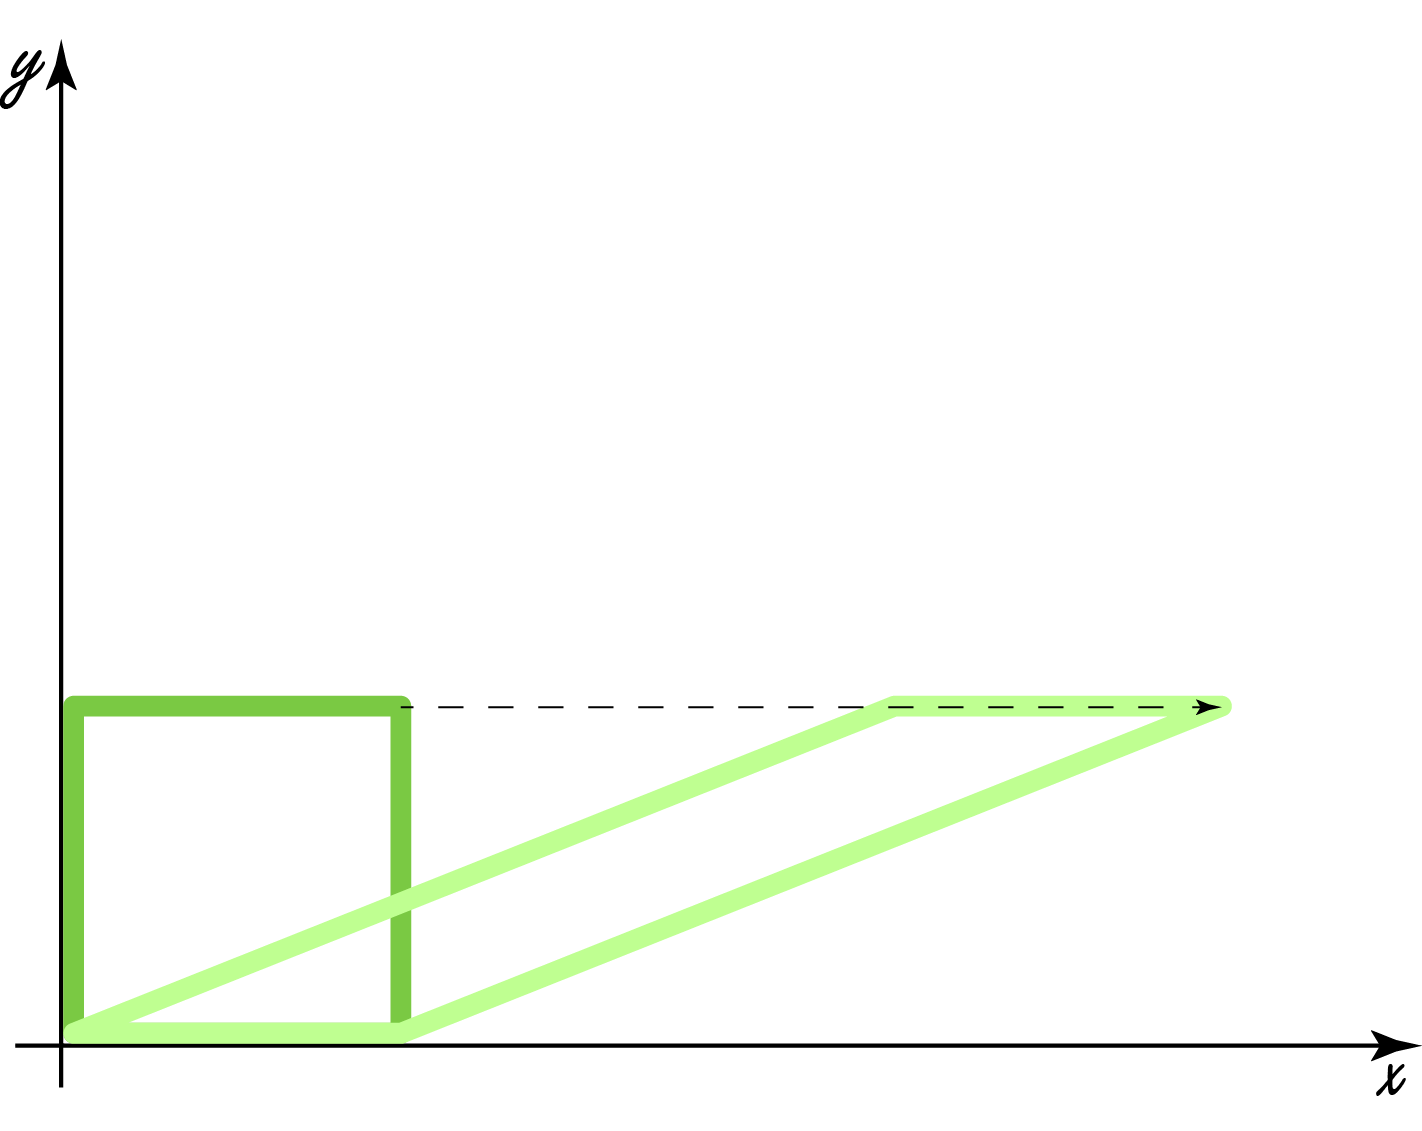
\includegraphics[scale=0.25]{figuras/shear1}
\caption{Exemplo de cisalhamento em um espaço bidimensional}
\end{center}
\end{figure}

\subsubsection{Projeção}
Projeção é o processo no qual se obtém uma figura bidimensional a partir de uma cena tridimensional.\cite{CGPPBook1}


\begin{center}
$\begin{bmatrix}x\\
y\\
z\\
\frac{z}{d}
\end{bmatrix}=\begin{bmatrix}1 & 0 & 0 & 0\\
0 & 1 & 0 & 0\\
0 & 0 & 1 & 0\\
0 & 0 & \frac{1}{d} & 0
\end{bmatrix}\begin{bmatrix}x\\
y\\
z\\
1
\end{bmatrix}$\end{center}

\begin{figure}[H] 
\begin{center}
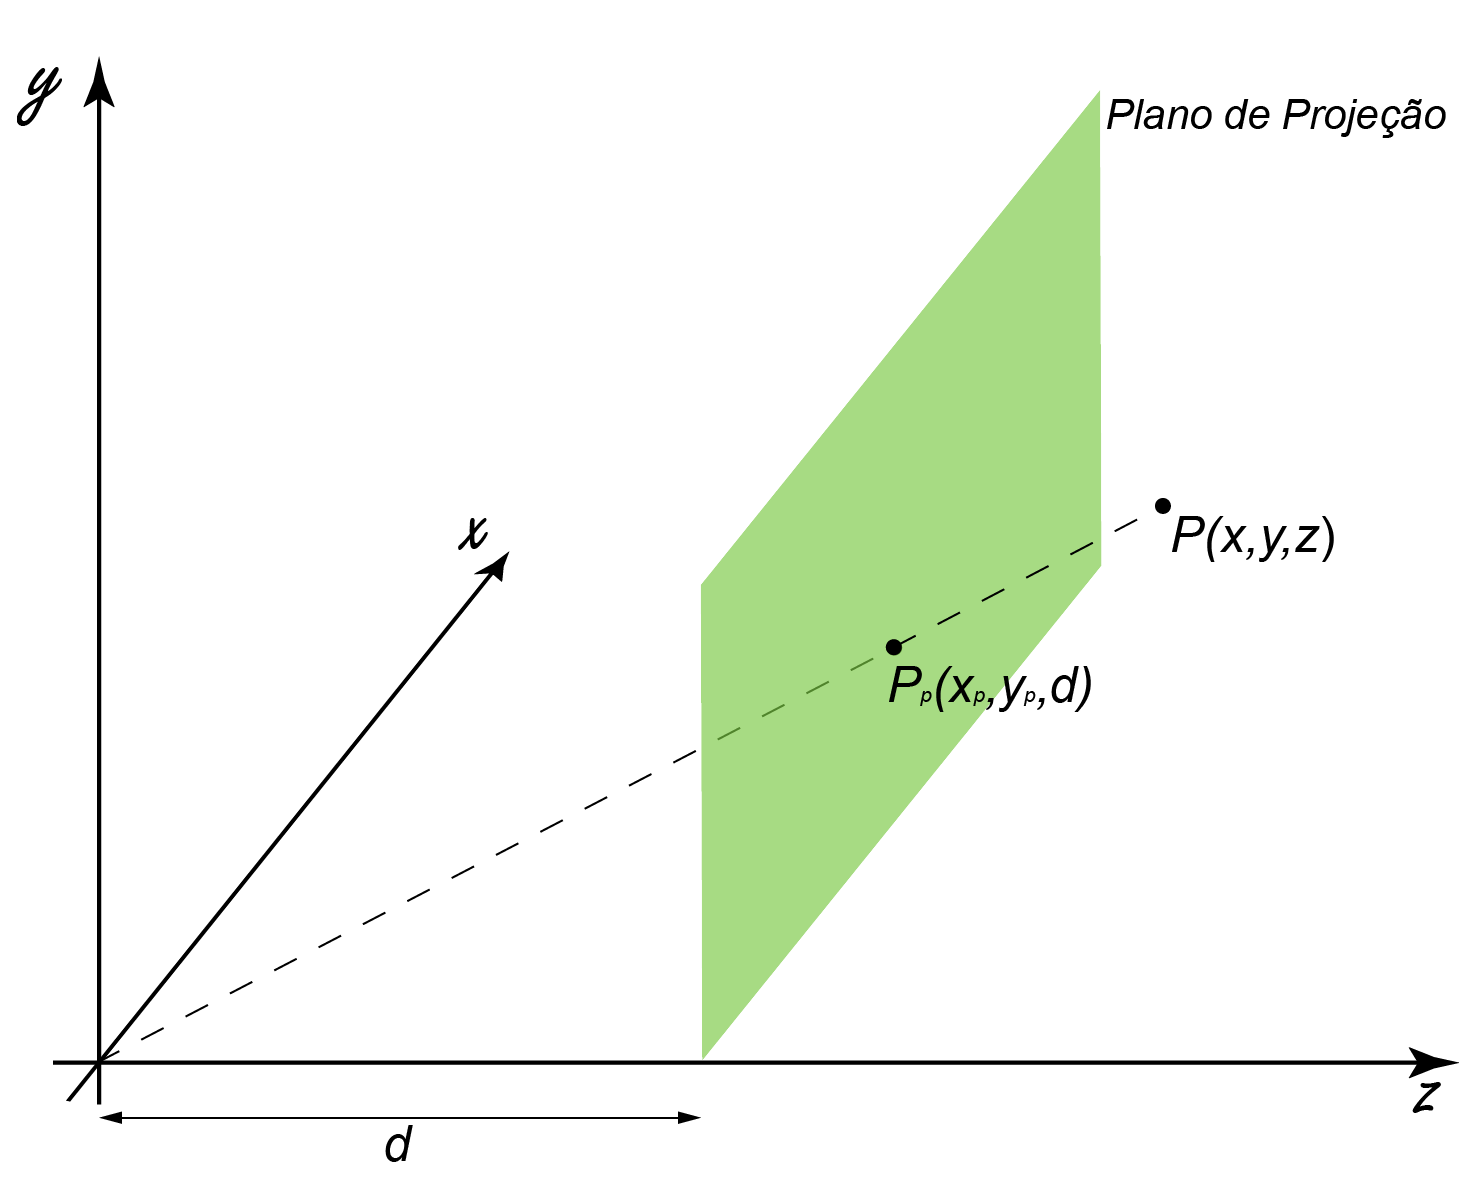
\includegraphics[scale=0.25]{figuras/projection1}
\caption{Exemplo de projeção}
\end{center}
\end{figure}

\subsection{Tipos de transformação}
É necessário primeiramente 
\subsubsection{Linear}
A transformação linear ou também chamada de euclidiana, pode ser definida como:
\begin{center}
$F(x)=Qx$\end{center}
Sendo que $Q=n\times m$.
Ou seja, transformações do tipo lineares são aquelas obtidas através de mutliplicações matriciais.
Assim, através das transformações lineares pode-se realizar operações de rotação, cisalhamento e variação de escala.\cite{CGPPBook1}
\subsubsection{Afim}
A transformação Afim é uma transformação que compreende as operações que a transformação linear
consegue executar mais a operação de translação. A transformada em questão pode ser definida como:

\begin{center}
$F(x)=Qx+q$\end{center}
Sendo que $Q=n\times m$ e $q$ tem tamanho $m$. \cite{CGPPBook1}

\subsubsection{Polinômio Segundo Grau}
Existe também transformações de segundo grau que são descritas como:
\begin{center}
$F(x)=a_{0}+a_{1}x+a_{2}y+a_{3}xy+a_{4}x^{2}+a_{5}y^{2}$\end{center}

\subsubsection{Projeção}

A projeção é nada mais que uma transformação linear em um espaço projetivo.\cite{CGPPBook1}
A forma geral da transformação projetiva é descrita como:

$F(x)=\left( \frac{a_{11}x_{1}+a_{12}x_{2}+...+a_{1n}x_{n}+a_{1n}x_{1(n+1)}}{b_{1}x_{1}+b_{2}x_{2}+...+b_{n}x_{n}+b_{n+1}},\cdots,\right.$

\begin{center}
$\left. \frac{a_{m1}x_{1}+a_{m2}x_{2}+...+a_{mn}x_{n}+a_{mn}x_{m(n+1)}}{b_{1}x_{1}+b_{2}x_{2}+...+b_{n}x_{n}+b_{n+1}} \right)$\end{center}



\section{Avaliação da Precisão do Registro}
Uma operação importante para um sistema de registro é a avaliação da transformação computada. Sejam {g} e {G} as imagens de ajuste e referência respectivamente, e {x, y} e {X, Y} os conjuntos de pontos de controle casados que definem uma transformação de distorção {T}. Podemos verificar o quão a transformação é correta através do cálculo do erro RMSE.

$$
	RMSE = \sqrt{\frac{1}{n}\sum\limits_{i=1}^{n}(x_i - T(X_i))^2 + (y_i - T(Y_i))^2}
$$

onde:

$(x_i, y_i), (X_i, Y_i)$, $i = 1..n$ é o conjunto de pares de pontos de contole obtidos no processo de casamento.
$T$ é a função de distorção entre as imagens obtida através do casamento de pontos de controle.



\section{ Fluxograma para gerar o Mosaico}
 A montagem do mosaico se baseia em duas classes do TerraLib, o arquivo MMIOMatching recebe duas imagens e apresenta como resultado os pontos de controle da cena, que são representados através de dois vetores para calculo da função de transformação. Esses pontos localizados são acrescentados na imagem que é salva com outro nome.
(Talvez colocar algo da dissetação do Dmitri Fedorov)
 Já o segundo arquivo  Mosaic recebe como entrada  a saida do  arquivo MMIOMatching, ou seja, os vetores  que representam os pontos de controle, além das imagens que serão mosaicadas e o nome da nova imagem.
(Devemos definir as configurações nesse item, qual foi a função de transformação que usamos entre outros detalhes, seria interessante fazer um desenho com explicando esse clico)

\section{Resultados}
Devemos descrever quanto tempo levou para executar, quantas imagens foram utilizadas para gerar o mosaico, quais as vantagens. 

\section{Comparação dos algoritmos}
Comparação do SIFT e dos algoritmos do TerraLib

\section{Conclusão}
Conclusão aqui.

\bibliographystyle{IEEEbib}
\bibliography{biblio}

\end{document}
